\chapter{Methodology}

The equipment needed and procedures undertaken to carry out 3D printing  are described in the following sections. The experiment was done at iPIC (Rapid Prototyping lab) in JKUAT.
\section{Equipment}
\begin{enumerate}
\item 3D Scanning hardware and software (Artec3D, Artec Spider, Artec Studio.)
\item Workpiece shown in Figure 3.1.1.
\item 3D Printing hardware and software ( )
\end{enumerate}
\begin{center}
	\begin{figure}[!h]
	\centering
	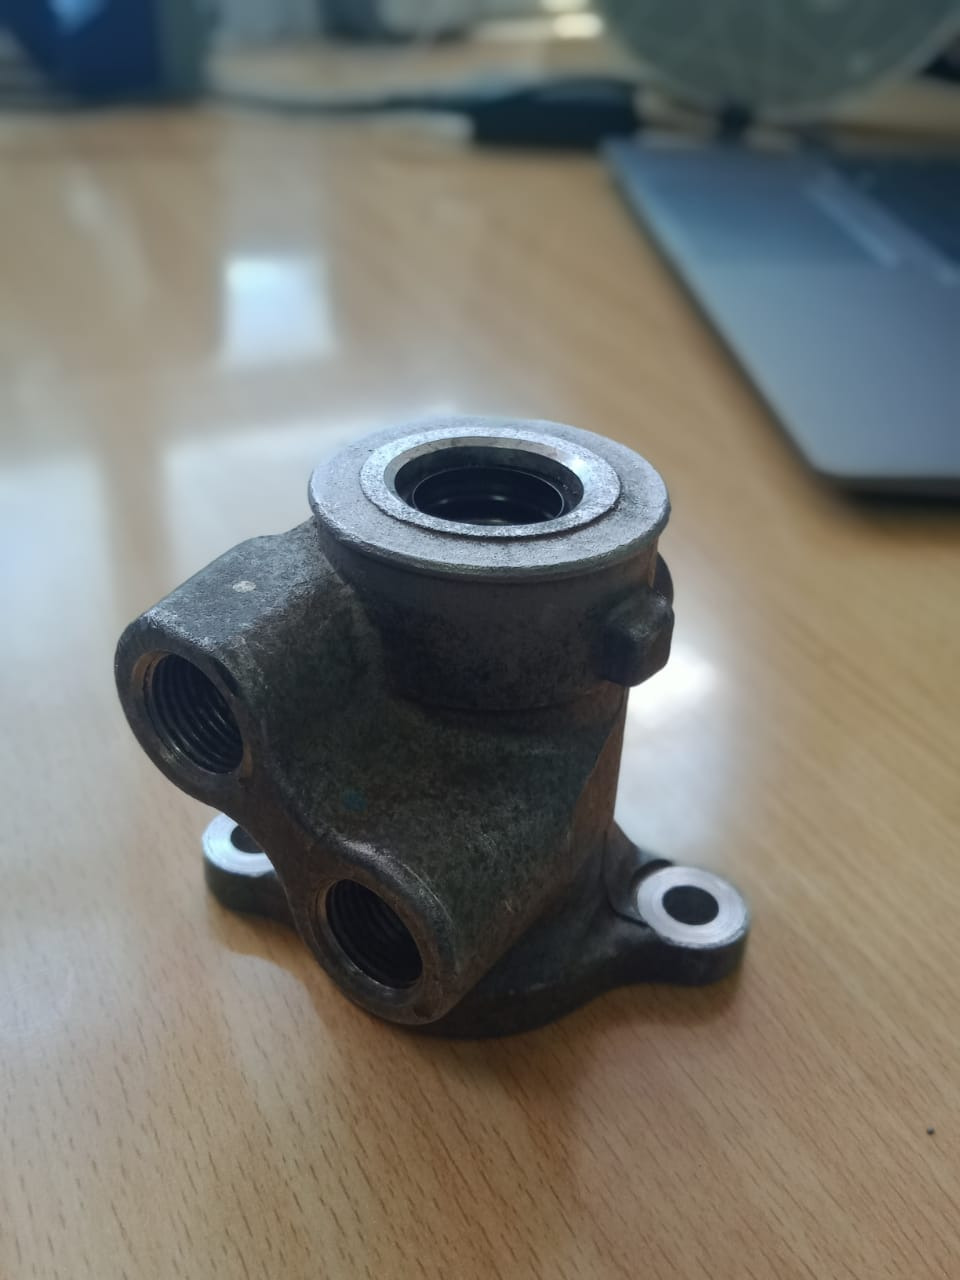
\includegraphics[width=0.5\linewidth]{Figures/Figure}
	\caption{Complex Workpiece}
	\end{figure}
\end{center}
\section{Procedure}
The 3D scanning hardware and software were set up and the workpiece placed on the turntable for scanning. Figure 3.2.1 shows the workpiece being scanned. Several scans were performed and the final 3D model was obtained. Figure 3.2.2 shows the 3D model obtained from the scans.
\begin{center}
 	\begin{figure}[!h]
 	\centering
 	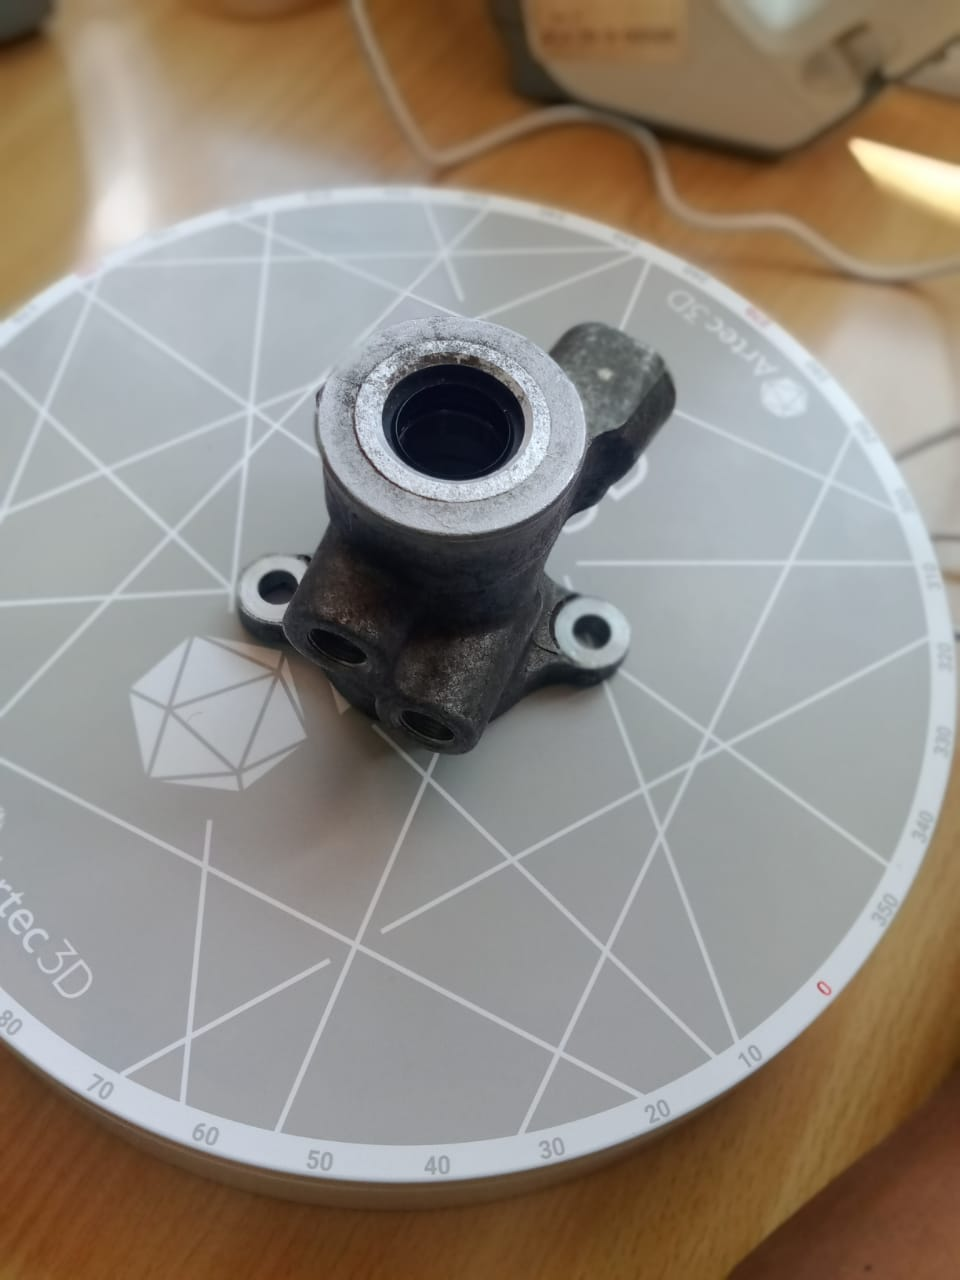
\includegraphics[width=0.4\linewidth]{Figures/Figure 2}
 	\caption[Scanning]{Workpiece being scanned}
 	\end{figure}
 \end{center}
 \begin{center}
 	\begin{figure}[!h]
 	\centering
 	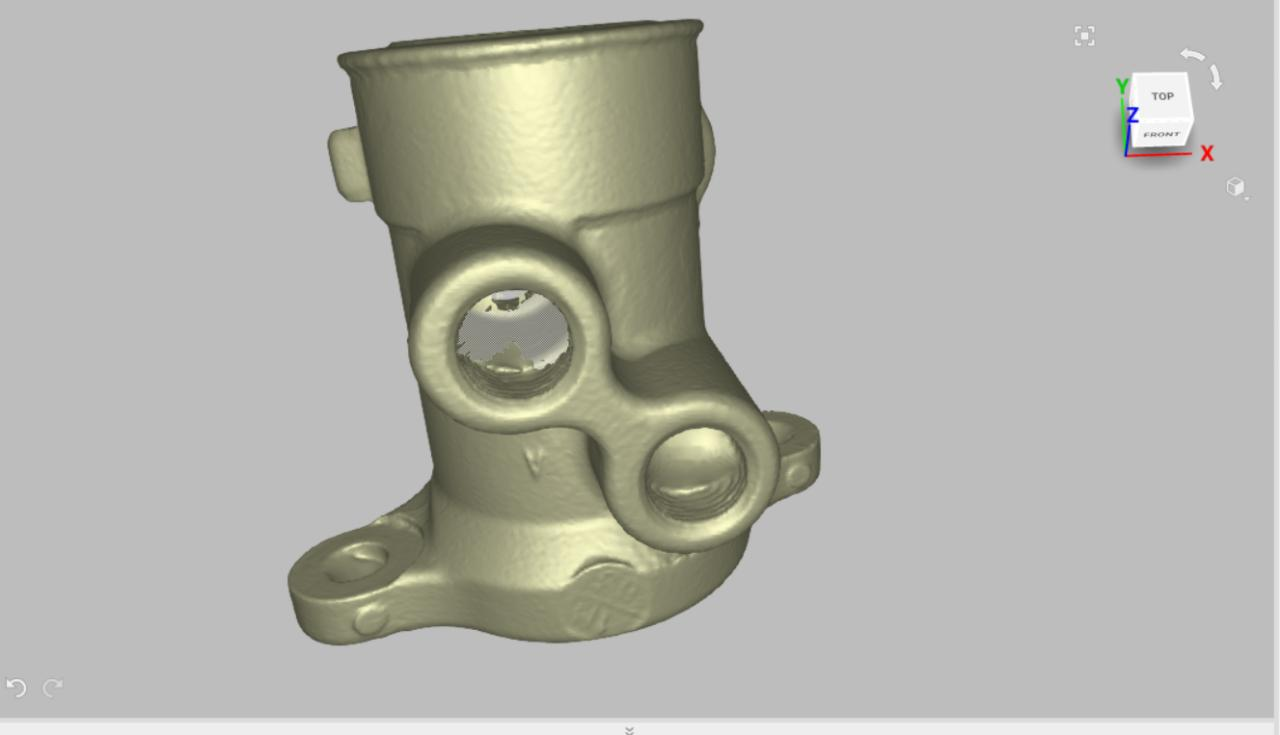
\includegraphics[width=0.8\linewidth]{Figures/Figure 1}
 	\caption[Scanned 3D model]{Model obtained from 3D scanning}
 	\end{figure}
 \end{center}
 